
\begin{subsection}{Diagrama de contexto}
En la figura \ref{fig:diagrama_contexto} puede verse el diagrama de contexto el cual, captura todos los agentes y fenómenos relativos al sistema anteriormente descripto.

\begin{figure}[!ht]
\begin{center}
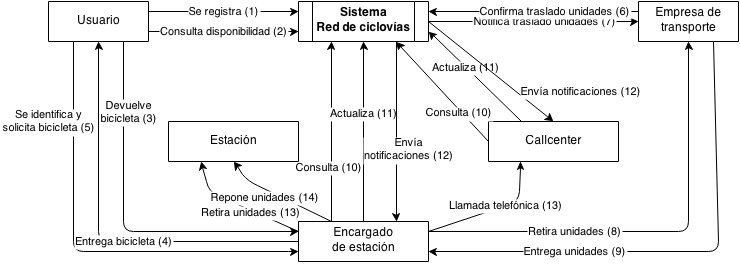
\includegraphics[scale=0.60]{imagenes/diagrama_contexto.png}
\caption{diagrama de contexto}
\label{fig:diagrama_contexto}
\end{center}
\end{figure}
\end{subsection}

\begin{subsection}{Agentes}
	\begin{itemize}
	\item Usuario.
	\item Encargado de estación.
	\item Callcenter.
	\item Estación.
	\item Empresa de transporte.
	\end{itemize}
\end{subsection}

\begin{subsection}{Eventos}

\textit{(Formato: Nro. de evento- Evento. \{Nro. de interacción entre agentes en el diagrama\})}

	\begin{itemize}
	\item [1-] EL USUARIO se registra por internet con el SISTEMA. \{\textbf{1}\}
	\end{itemize} 

\end{subsection}